
	\section{The Framework}
	Our framework \clusteval is intended to perform automatized cluster analysis of arbitrary datasets and clustering methods. The goal is, that any clustering method known to the framework can be applied to any known dataset (with certain exceptions, partly inflicted by the clustering methods itself and partly inflicted by the framework constraints).
	
	In general \clusteval is divided into a backend and a frontend. Figure \ref{fig_general_structure} shows the general structure of the framework. The backend is reponsible for doing all the calculations including clusterings and the frontend has only visualization purposes.

\begin{figure}[hbtp]
\caption{General framework flow}
\label{fig_general_structure}
\centering
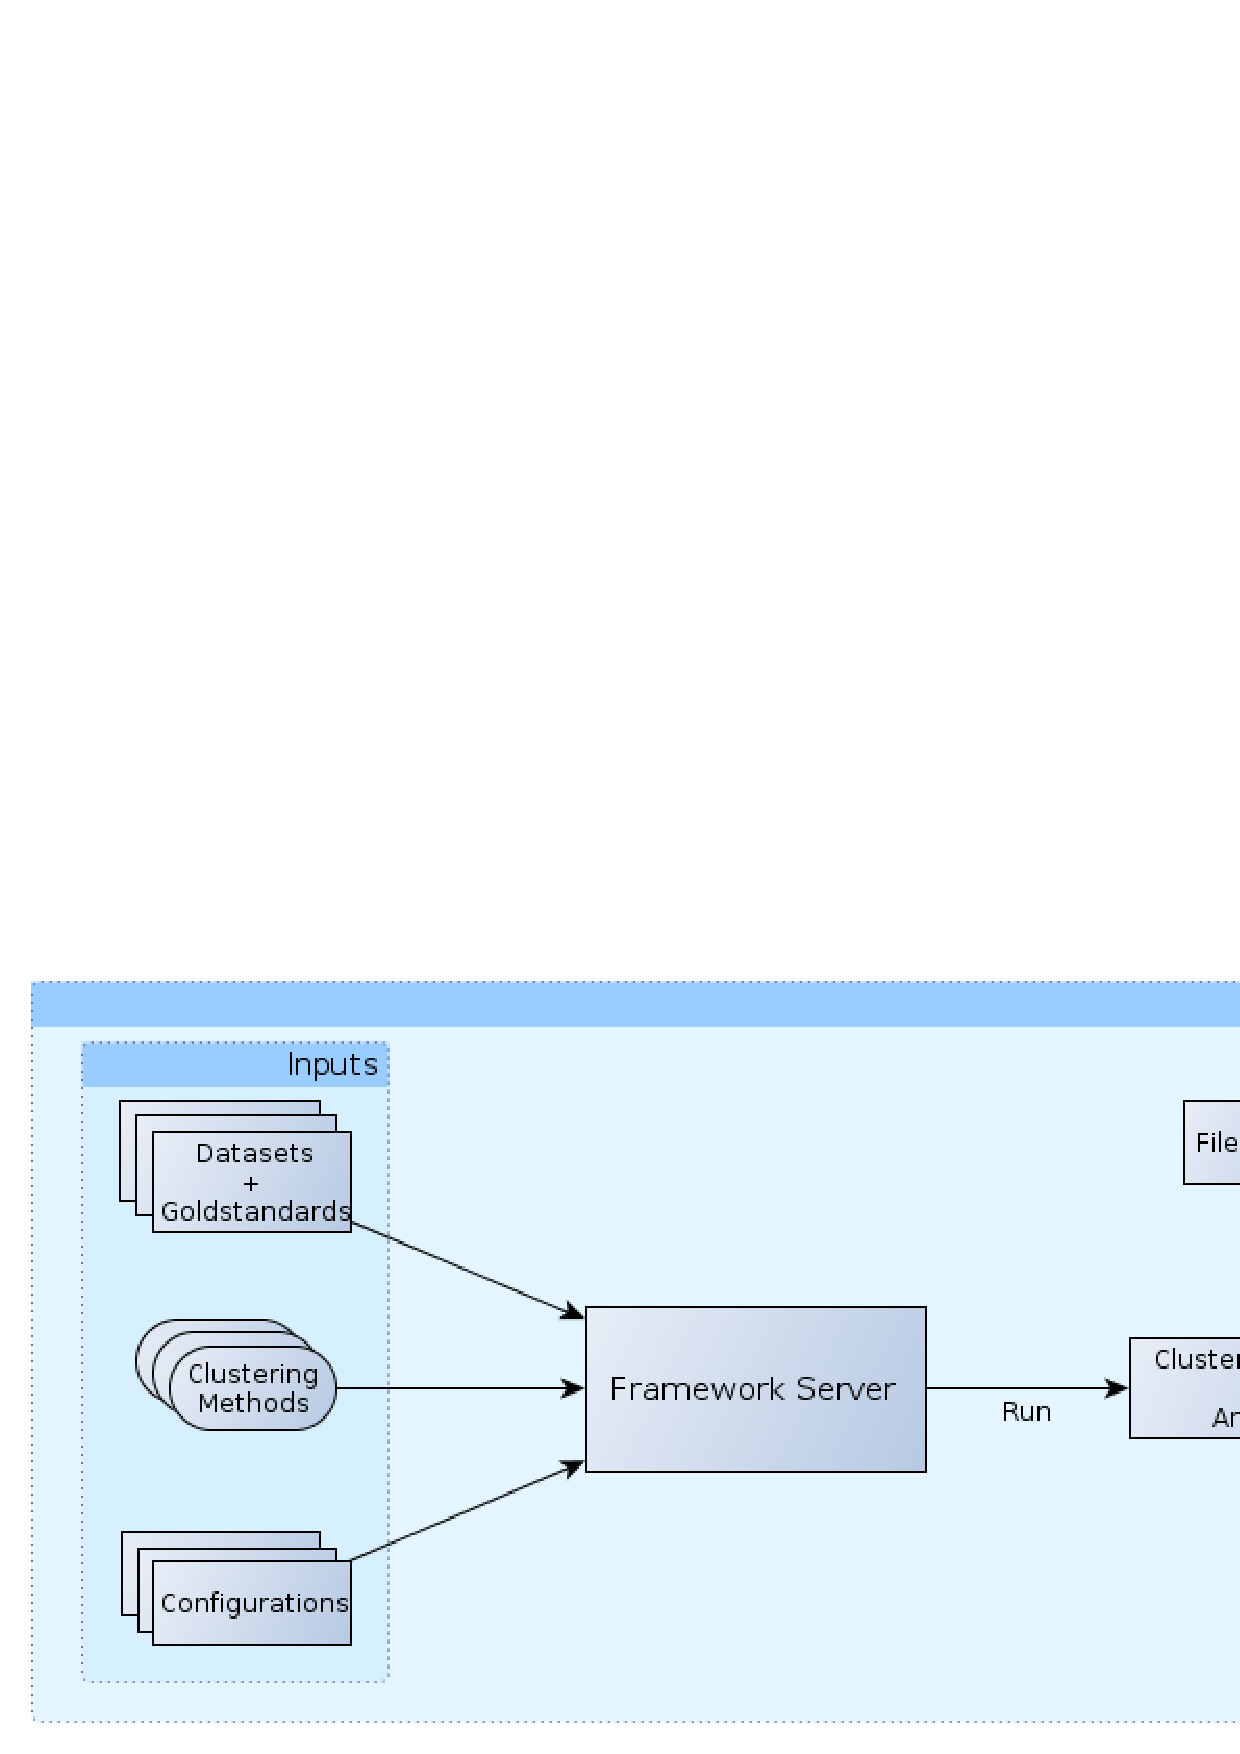
\includegraphics[width=\textwidth]{../master_seminar_presentation/framework_flow.png}
\end{figure} 

At first we will give an overview of the backend in \ref{subsec_general_backend} and then of the frontend in \ref{subsec_general_frontend}.